\chapter{2013}

\section{01}
\subsection{31/01/13}
\begin{itemize}
\item Presentación de la Asignatura
\item Ejercicio: \htmladdnormallink{Darse de alta en la comunidad de google plus
PL Grado ULL 12/1}{https://plus.google.com/u/0/communities/100856772699690495413"}
\item Ejercicio: Indicar un mail en gmail para compartir recursos
\item Ejercicio: Indicar página en GitHub
\end{itemize}

\section{03}

\subsection{Repaso 07/03/13}

\begin{enumerate}

\item
¿Que retorna?
\begin{verbatim}
"hello small world and blue sky".match(/(\S+)\s+(\S+)/);
\end{verbatim}

\item
Indique que casa con el primer paréntesis y que con el segundo en las siguientes expresiones regulares:
\begin{verbatim}
> x = "I have 2 numbers: 53147"
> pats = [ /(.*)(\d*)/, 
           /(.*)(\d+)/, 
           /(.*?)(\d*)/, 
           /(.*?)(\d+)/, 
           /(.*)(\d+)$/, 
           /(.*?)(\d+)$/, 
           /(.*)\b(\d+)$/, 
           /(.*\D)(\d+)$/ ]
\end{verbatim}
Es decir, compute la salida de:
\begin{verbatim}
   pats.map( function(r) { return r.exec(x).slice(1); })
\end{verbatim}
\item
¿Que retorna el matching?:
\begin{verbatim}
>  a = "hola juan"
 => "hola juan" 
> a.match(/(?:hola )*(juan)/)
\end{verbatim}
\item ¿Que salidas se obtienen?
\begin{verbatim}
> "a\na".match(/a$/)
________________________________
> "a\na".match(/a$/m)
________________________________
> "a\na".match(/^a/gm)
____________
> "a\na".match(/^a/g)
_______
\end{verbatim}
\item
Escriba  la expresión regular que da lugar a este resultado (enumerar las líneas):
\begin{verbatim}
> x = "one\ntwo\nthree\nfour"
'one\ntwo\nthree\nfour'
> a = (c = 1, x.replace(_____, function(t) { return  c++ + ' ' + t; }))
'1 one\n2 two\n3 three\n4 four'
> console.log(a)
1 one
2 two
3 three
4 four
undefined
\end{verbatim}
\item
Supongamos dado el método
\begin{verbatim}
String.prototype.repeat = function( num ) {
    return new Array( num + 1 ).join( this );
}
\end{verbatim}
de manera que podamos escribir expresiones como:
\begin{verbatim}
> x = 'a'.repeat(40)
'aaaaaaaaaaaaaaaaaaaaaaaaaaaaaaaaaaaaaaaa'
\end{verbatim}
Encontremos una solución de la ecuación diofántica \verb|3x + 2y + 5z = 40|
\begin{verbatim}
> m = x.match(/^_______________________________$/).slice(1)
[ 'aaaaaaaaaaaaaaaaaaaaaaaaaaaaaaaaa',
  'aa',
  'aaaaa' ]
\end{verbatim}
Calculemos las longitudes de las tres cadenas:
\begin{verbatim}
> r = m.map(function(s) { return s.length; })
[ 33, 2, 5 ]
\end{verbatim}
Dividamos por los coeficientes para obtener la solución:
\begin{verbatim}
> coef = [3, 2, 5]
> i = 0; w = r.map(function(x) { return x/coef[i++]; }
[ 11, 1, 1 ]
\end{verbatim}
Encuentre la expresión regular usada.
\item 
Escriba una expresión regular que reconozca cadenas de dobles comillas como \verb|"hello world"|
y en las que las comillas puedan aparecer escapadas como en \verb|"Hello \"Jane\" and Jakes"|

\item
Escriba una expresión regular que reconozca los números en punto flotante como
\verb|2.34|, \verb|-5.2e-1| y \verb|0.9e3|

\item
\label{item:ccomments}
¿Que queda en \verb|m[0]|?
\begin{verbatim}
m = 'main() /* 1c */ { /* 2c */ return; /* 3c */ }'.match(new RegExp('/\\*.*\\*/'))
\end{verbatim}
¿Por qué?
\item 
¿Por qué debemos duplicar el carácter de escape \verb|\| en  la expresión regular \verb|new RegExp('/\\*.*\\*/')| de la pregunta anterior \ref{item:ccomments}?
\item
Se quiere poner un espacio en blanco después de la aparición de cada coma:
\begin{verbatim}
> 'ab,cd,4,3,   de,   fg'.replace(/,/, ', ')
=> "ab, cd, 4, 3,    de,    fg" 
\end{verbatim}
pero se quiere que la sustitución no tenga lugar si la coma esta incrustada entre
dos dígitos. Además se pide que si hay ya un espacio después de la coma,
no se duplique

Como función de reemplazo use:
\begin{verbatim}
f = function(match, p1, p2, offset, string) { return (p1 || p2 + " "); }
\end{verbatim}

\item
Escribe un patrón regular
que reconozca las cadenas  que representan números no primos en unario
de manera que el primer paréntesis case con el divisor mas grande del número.

\item
Escribe un patrón regular
que reconozca las cadenas  que representan números no primos en unario
de manera que el primer paréntesis case con el divisor mas pequeño del número.

\item Escriba una expresión regular que reconozca los comentarios del lenguaje JavaScript de la forma
\verb|// ...  |

\item Escriba una expresión regular que reconozca los comentarios del lenguaje JavaScript de la forma
\verb|/* ...  */|


\item Rellene lo que falta para que la salida sea la que aparece en la sesión de node:
\begin{verbatim}
> re = __________
> str = "John Smith"
'John Smith'
> newstr = str.replace(re, "______")
'Smith, John'
\end{verbatim}
\item  Rellene las partes que faltan:
\begin{verbatim}
> re = /d(b+)(d)/ig
/d(b+)(d)/gi
> z = "dBdxdbbdzdbd"
'dBdxdbbdzdbd'
> result = re.exec(z)
[ ______, _____, ______, index: __, input: 'dBdxdbbdzdbd' ]
> re.lastIndex
______
> result = re.exec(z)
[ ______, _____, ______, index: __, input: 'dBdxdbbdzdbd' ]
> re.lastIndex
______
> result = re.exec(z)
[ ______, _____, ______, index: __, input: 'dBdxdbbdzdbd' ]
> re.lastIndex
______
> result = re.exec(z)
_____
\end{verbatim}
\item Escriba la expresión regular \verb|r| para que produzca el resultado final:
\begin{verbatim}
> x = "hello"
> r = /l(___)/
> z = r.exec(x)
[ 'l', index: 3, input: 'hello' ]
\end{verbatim}
\item 
\begin{verbatim}
> z = "dBdDBBD"
> re = /d(b+)(d)/ig
> re.lastIndex = ________
> result = re.exec(z)
[ 'DBBD',
  'BB',
  'D',
  index: 3,
  input: 'dBdDBBD' ]
\end{verbatim}
\item  Conteste:
\begin{enumerate}
\item Explique que hace el siguiente fragmento de código:
\begin{verbatim}
> RegExp.prototype.bexec = function(str) {
...   var i = this.lastIndex;
...   var m = this.exec(str);
...   if (m && m.index == i) return m;
...   return null;
... }
[Function]
\end{verbatim}
\item Rellene las salidas que faltan:
\begin{verbatim}
> re = /d(b+)(d)/ig
/d(b+)(d)/gi
> z = "dBdXXXXDBBD"
'dBdXXXXDBBD'
> re.lastIndex = 3
> re.bexec(z)
_____________________________________________________
> re.lastIndex = 7
> re.bexec(z)
_____________________________________________________
\end{verbatim}
\end{enumerate}
\item 
Escriba una expresión JavaScript que permita reemplazar todas las apariciones de palabras repetidas en una String por una sóla aparición de la misma
\item 
Supongamos que se usa una función como segundo argumento de \verb|replace|.
¿Que argumentos recibe?
\item 
¿Cual es la salida?
\begin{verbatim}
> "bb".match(/b|bb/)

> "bb".match(/bb|b/)

\end{verbatim}

\item  El siguiente fragmento de código tiene por objetivo
escapar las entidades HTML para que no sean intérpretadas como código HTML.
Rellene las partes que faltan.
\begin{verbatim}
var entityMap = {
    "&": "&___;",
    "<": "&__;",
    ">": "&__;",
    '"': '&quot;',
    "'": '&#39;',
    "/": '&#x2F;'
  };

function escapeHtml(string) {
  return String(string).replace(/_________/g, function (s) {
    return ____________;
  });
\end{verbatim}
\item ¿Cual es la salida?
\begin{verbatim}
> a = [1,2,3]
[ 1, 2, 3 ]
> b = [1,2,3]
[ 1, 2, 3 ]
> a == b
________
\end{verbatim}
\item
¿Como se llama el método que permite obtener una representación como cadena de un objeto?
¿Que parámetros espera? ¿Como afectan dichos parámetros?
\item ¿Cual debe ser el valor del atributo \verb|rel| para usar la imagen como favicon?
\begin{verbatim}
<link rel="_____________" href="etsiiull.png" type="image/x-icon"> 
\end{verbatim}
\item
Escriba un código JavaScript que defina una clase \verb|Persona| con atributos \verb|nombre|
y \verb|apellidos| y que disponga de un método \verb|saluda|.
\item
Reescriba la solución al problema anterior haciendo uso del método \verb|template|
de  \verb|underscore| y ubicando el template dentro de un tag \verb1script1.
\item Rellene lo que falta:
\begin{verbatim}
[~/srcPLgrado/temperature/tests(master)]$ cat tests.js 
var assert = chai.______;

suite('temperature', function() {
    test('[1,{a:2}] == [1,2]', function() {
      assert._________([1, {a:2}], [1, {a:2}]);
    });
    test('5X = error', function() {
        original.value = "5X";
        calculate();
        assert._____(converted.innerHTML, /ERROR/);
    });
});
\end{verbatim}
% \item añadir sinatra app
\item
¿Cómo se llama el directorio por defecto desde el que una aplicación sinatra sirve los ficheros estáticos?
\item
Explique la línea:
\begin{verbatim}
set :public_folder, File.dirname(__FILE__) + '/starterkit'
\end{verbatim}
¿Que es \verb|__FILE__|? ¿Que es \verb|File.dirname(__FILE__)|?
¿Que hace el método \verb|set|? (Véase 
\htmladdnormallink{http://www.sinatrarb.com/configuration.html}{http://www.sinatrarb.com/configuration.html})
% takes a setting name and value and creates an attribute on the application object
\item Escriba un programa sinatra que cuando se visite la URI \verb|/chuchu| muestre
una página que diga \verb|"hello world!"|
\item
¿Cual es el signifcado de \verb|__END__| en un programa Ruby?
\item  
\label{sinatalayout}
Esta y las preguntas 
\ref{sinatraindex} y
\ref{sinatrachuchu} se refieren al mismo programa ruby sinatra.
Explique este fragmento de dicho programa ruby sinatra. 
\begin{verbatim}
@@layout
  <!DOCTYPE html>
  <html>
    <head>
        <meta charset="utf-8" />
        <title>Demo</title>
    </head>
    <body>
        <a href="http://jquery.com/">jQuery</a>
        <div class="result"></div>
        <script src="jquery.js"></script>
        <%= yield %>
    </body>
  </html>
\end{verbatim}
\begin{enumerate}
\item ¿En que lugar del fichero que contiene el programa está ubicada esta sección? 
\item ¿Cómo se llama el lenguaje en el que esta escrita esta sección?
\item ¿Para que sirve la sección \verb|layout|?
\item ¿Cual es la función del \verb|<div class="result"></div>|?
\item ¿Para que sirve el \verb|<%= yield %>|?
\end{enumerate}
\item 
\label{sinatraindex}
Explique este fragmento de un programa ruby sinatra.
\begin{verbatim}
@@index
  <script>
  $( document ).ready(function() {
      $( "a" ).click(function( event ) {
          event.preventDefault();
          $.get( "/chuchu", function( data ) {
            $( ".result" ).html( data );
            alert( "Load was performed." );
          });
      });
  });
  </script>
\end{verbatim}
\begin{enumerate}
\item ¿Cuando ocurre el evento \verb|ready|?
\item ¿Que hace \verb|event.preventDefault()|?
\item ¿Que hace \verb|$.get( "/chuchu", function( data ) { ... }|?
¿Cuando se dispara la callback?
\item ¿que hace la línea \verb|$( ".result" ).html( data )|?
\end{enumerate}
% \item añadir jquery ajax
\item Explique este fragmento de código ruby-sinatra:
\label{sinatrachuchu}
\begin{verbatim}
get '/chuchu' do
  if request.xhr? 
    "hello world!"
  else 
    erb :tutu
  end
end
\end{verbatim}
\item  En el siguiente programa - que calcula la conversión
de temperaturas entre grados Farenheit y Celsius - rellene las partes que faltan:
\begin{enumerate}
\item  index.html:
\begin{verbatim}
<html>
  <head>
      <meta http-equiv="Content-Type" content="text/html; charset=_____">
      <title>JavaScript Temperature Converter</title>
      <link ____="global.css" ___="stylesheet" ____="text/css">

     <script type="_______________" src="temperature.js"></script>
  </head>
  <____>
    <h1>Temperature Converter</h1>
    <table>
      <tr>
        <th>Enter  Temperature (examples: 32F, 45C, -2.5f):</th>
        <td><input id="________" ________="calculate();"></td>
      </tr>
      <tr>
        <th>Converted Temperature:</th>
        <td><span class="output" id="_________"></span></td>
      </tr>
    </table>
  </____>
</html>
\end{verbatim}

\item Rellene las partes del código JavaScript que faltan en \verb|temperature.js|:
\begin{verbatim}
"use strict"; // Use ECMAScript 5 strict mode in browsers that support it
function calculate() {
  var result;
  var original       = document.getElementById("________");
  var temp = original.value;
  var regexp = /_______________________________/;
  
  var m = temp.match(______);
  
  if (m) {
    var num = ____;  // paréntesis correspondiente
    var type = ____;
    num = parseFloat(num);
    if (type == 'c' || type == 'C') {
      result = (num * 9/5)+32;
      result = ______________________________ // 1 sólo decimal y el tipo
    }
    else {
      result = (num - 32)*5/9;
      result = ____________________________ // 1 sólo decimal y el tipo
    }
    converted._________ = result; // Insertar "result" en la página
  }
  else {
    converted._________ = "ERROR! Try something like '-4.2C' instead";
  }
}
\end{verbatim}
\end{enumerate}
\item  ¿Que hace \verb|autofocus|?
\begin{verbatim}
<td><textarea autofocus cols = "80" rows = "5" id="original"></textarea></td> 
\end{verbatim}
\item  ¿Que hacen las siguientes pseudo-clases estructurales CSS3?
\begin{verbatim}
tr:nth-child(odd)    { background-color:#eee; }
tr:nth-child(even)    { background-color:#00FF66; }
\end{verbatim}
\item ¿Que contiene el objeto \verb|window| en un programa JavaScript que se ejecuta en un navegador?

\item 
\begin{enumerate}
\item 
¿Que es \htmladdnormallink{Local Storage}{http://diveinto.html5doctor.com/storage.html}? ¿Que hace la siguiente línea?
\begin{verbatim}
  if (window.localStorage) localStorage.original  = temp;
\end{verbatim}
\item  ¿Cuando se ejecutará esta callback? ¿Que hace?
\begin{verbatim}
window.onload = function() {
  // If the browser supports localStorage and we have some stored data
  if (window.localStorage && localStorage.original) {
    document.getElementById("original").value = localStorage.original;
  }
};
\end{verbatim}
\end{enumerate}

\item  ¿Cómo se hace para que elementos de la página web permanezcan ocultos para 
posteriormente mostrarlos? ¿Que hay que hacer en el HTML, en la hoja de estilo y en el JavaScript?
\item Rellene los estilos para los elementos de las clases para que su visibilidad
case con la que su nombre indica:
\begin{verbatim}
.hidden      { display: ____; }
.unhidden    { display: _____; }
\end{verbatim}
\item 
Los siguientes textos corresponden  a los ficheros de 
la práctica 
de construcción de un analizador léxico de los ficheros de configuración INI. 
Rellena las partes que faltan.
\begin{enumerate}
\item  Rellena las partes que faltan en el contenido del fichero \verb|index.html|. 
Comenta que hace el tag \verb|<input>|.
Comenta que hace el tag \verb|<pre>|.
\begin{verbatim}
<html>
  <head>
     <meta http-equiv="Content-Type" content="text/html; charset=UTF-8">
     <title>INI files</title>
     <link href="global.css" rel="__________" type="text/css">

     <script type="_______________" src="underscore.js"></script>
     <script type="_______________" src="jquery.js"></script>
     <script type="_______________" src="______"></script>
  </head>
  <body>
    <h1>INI files</h1>
    <input type="file" id="_________" />
    <div id="out" class="hidden">
    <table>
      <tr><th>Original</th><th>Tokens</th></tr>
      <tr>
        <td>
          <pre class="input" id="____________"></pre>
        </td>
        <td>
          <pre class="output" id="___________"></pre>
        </td>
      </tr>
    </table>
    </div>
  </body>
</html>
\end{verbatim}

\item 
A continuación siguen los contenidos del fichero \verb|ini.js| conteniendo el JavaScript.
\begin{enumerate}
\item 
Rellena las partes que faltan. 
El siguiente ejemplo de fichero \verb|.ini| le puede ayudar
a recordar la parte de las expresiones regulares 
\begin{verbatim}
; last modified 1 April 2001 by John Doe
[owner]
name=John Doe
organization=Acme Widgets Inc.
\end{verbatim}
\item 
Explica 
el uso del template.
\item 
Explica el uso de JSON.stringify
\end{enumerate}
\begin{verbatim}
"use ______"; // Use ECMAScript 5 strict mode in browsers that support it

$(document)._____(function() {
   $("#fileinput").______(calculate);
});

function calculate(evt) {
  var f = evt.target.files[0]; 

  if (f) {
    var r = new __________();
    r.onload = function(e) { 
      var contents = e.target.______;
      
      var tokens = lexer(contents);
      var pretty = tokensToString(tokens);
      
      out.className = 'unhidden';
      initialinput._________ = contents;
      finaloutput._________ = pretty;
    }
    r.__________(f); // Leer como texto
  } else { 
    alert("Failed to load file");
  }
}

var temp = '<li> <span class = "<%= ______ %>"> <%= _ %> </span>\n';

function tokensToString(tokens) {
   var r = '';
   for(var i in tokens) {
     var t = tokens[i];
     var s = JSON.stringify(t, undefined, 2); //______________________________
     s = _.template(temp, {t: t, s: s});
     r += s;
   }
   return '<ol>\n'+r+'</ol>';
}

function lexer(input) {
  var blanks         = /^___/;
  var iniheader      = /^________________/;
  var comments       = /^________/;
  var nameEqualValue = /^________________________/;
  var any            = /^_______/;

  var out = [];
  var m = null;

  while (input != '') {
    if (m = blanks.____(input)) {
      input = input.substr(m.index+___________);
      out.push({ type : ________, match: _ });
    }
    else if (m = iniheader.exec(input)) {
      input = input.substr(___________________);
      _______________________________________ // avanzemos en input
    }
    else if (m = comments.exec(input)) {
      input = input.substr(___________________);
      _________________________________________
    }
    else if (m = nameEqualValue.exec(input)) {
      input = input.substr(___________________);
      _______________________________________________
    }
    else if (m = any.exec(input)) {
      _______________________________________
      input = '';
    }
    else {
      alert("Fatal Error!"+substr(input,0,20));
      input = '';
    }
  }
  return out;
}
\end{verbatim}
\end{enumerate}


\end{enumerate}

\section{04}

\subsection{Repaso 18/04/13}

\begin{enumerate}

\item
Escriba un analizador léxico en Jison 
(que suponemos se guardará en un fichero \verb|calc.l|) 
para una calculadora con números, restas, productos y menos unario

\item
\label{item:grammar}
Escriba el correspondiente analizador sintáctico en Jison 
(que suponemos se guardará en un fichero \verb|calc.jison|) 
para una calculadora con números, productos, restas y menos unario.
Deberá aceptar frases como \verb|-2.5|, \verb|-3.1e2-5e3|, \verb|-2*3|,
etc.


\item
Añada acciones semánticas a 
la gramática del ejercicio 
\ref{item:grammar}
para la evaluación de las expresiones
aritméticas. Puede contestar conjuntamente a este ejercicio 
y al ejercicio \ref{item:grammar} 

\item 
Explique que conflictos aparecen en el 
ejercicio
\ref{item:grammar} y como los ha resuelto
¿Cómo se resuelven los conflictos en yacc?
¿Cómo se da precedencia a las reglas y a los terminales?

\item 
Escriba el comando para generar el código javascript de la mini
calculadora a partir de los fuentes \verb|calc.jison| y
\verb|calc.l|

\item 
Calcule los FIRST para las variables sintácticas de dicha gramática
(Véase 
\ref{subsection:first})
\item 
Calcule los FOLLOW  para las variables sintácticas de dicha gramática
(Véase la sección
\ref{subsection:first})

\item
\label{item:dfa}
Calcule el DFA que reconoce los prefijos viables de dicha gramática
(Véase la sección 
\ref{section:conceptosbasicos}
y la sección
\ref{subsection:nfa2dfa})
\item 
Simule la antiderivacion a derechas/construción del árbol de análisis sintáctico
realizada usando el DFA construído en el ejercicio 
\ref{item:dfa}
sobre la 
entrada
'\verb|-1-2|'.

En cada momento de la simulación indique cual es la forma sentencial derecha actual y 
la posición en la misma (algo como $-e_\uparrow - NUM$),
en que posición de lectura de la entrada estamos 
(esto es, quién es el token lookahead que se está viendo), en que estado
del DFA estamos y cual es la acción tomada (desplazar o reducir).


\end{enumerate}

\subsection{Proyecto: Diseña e Implementa un Lenguaje de Dominio Específico}

Se trata de realizar un proyecto relacionado con el procesamiento de lenguajes.
El objetivo puede ser:


\begin{enumerate}
\item
Diseñar un lenguaje de dominio específico para simplificar cualquier tarea en la que estés interesado:

\begin{itemize}
\item
Para escribir exámenes, 
\item
Para dibujar árboles, 
\item
Para calcular fechas,
\item
Para generar emails
\item
Para escribir música
\item
Para escribir autómatas finitos
\item 
Para procesar 
\htmladdnormallink{CSS}{http://www.w3.org/TR/CSS21/grammar.html\#grammar}
\item
etc.
\end{itemize}
\item
Estudiar un traductor existente en profundidad  como:
\begin{itemize}
\item 
ECMAscript 5.1: 
\htmladdnormallink{Creating a JavaScript Parser}{http://cjihrig.com/blog/creating-a-javascript-parser/} Una implementación de ECMAScript 5.1 usando Jison 
disponible 
en GitHub
 en
\htmladdnormallink{https://github.com/cjihrig/jsparser}{https://github.com/cjihrig/jsparser}.
Puede probarse en:
\htmladdnormallink{http://www.cjihrig.com/development/jsparser/}{http://www.cjihrig.com/development/jsparser/}
\item Roy
\item CoffeScript
\item Jison
\item 
\htmladdnormallink{Javascript 1.4}{http://www-archive.mozilla.org/js/language/grammar14.html}
\item etc.
\end{itemize}
\item
También puedes proponer tu propio tema relacionado al profesor
\end{enumerate}

Se recomienda para ello organizar equipos de no menos de dos y no mas de cuatro.

Las presentaciones de los proyectos tendrán lugar el último día de clase Martes 21 de Mayo.


\section{05}

\subsection{Repaso 16/05/13}
\begin{enumerate}

\item
Esta gramática contiene un conflicto:

\begin{verbatim}
  %token D S

  %%
  p: ds ';' ss  | ss ;
  ds: D ';' ds    
    | D  
  ;
  ss: S ';' ss  | S  ;
  %% 
\end{verbatim}

\begin{itemize}
\item ¿En que consiste el conflicto?
\item
Reescriba la gramática para eliminar el conflicto
\end{itemize}


\item
\label{item:ambgrammar}
El siguiente lenguaje es intrínsecamente ambiguo y por tanto no puede ser completamente 
descrito por una gramática independiente del contexto:


 \[ \{ a^n b^n c^m : n \ge 0, m \ge 0 \} \cup \{ a^n b^m c^m : n \ge 0, m \ge 0 \} \]

Esto  es: Concatenaciones de repeticiones 
de $a$s seguidas de repeticiones de $b$s y seguidas de
repeticiones de $c$s donde el número
de $a$s es igual al número de $b$s
o bien el número de $b$s es igual al número de $c$s.

Escriba un programa Jison que reconozca este lenguaje.

\item 
Escriba un programa \verb|pegjs| que sin hacer uso de acciones semánticas
reconozca el lenguaje 
descrito en la pregunta
\ref{item:ambgrammar}.
Permita la presencia de blancos entre las letras \verb|a|, \verb|b| y \verb|c|.

\item 
Complete las partes de código que faltan 
en esta calculadora de expresiones aritméticas
escrita en pegjs-coffee:

\begin{verbatim}
{ 
  @reduce = (left, right)->  
    sum = left
    for t in right
      op = ____
      num = ____
      switch op 
        when '_' then __________
        when '_' then __________
        when '_' then __________
        when '_' then __________
        else _________________________
    sum
  
}
sum   = left:product _____:_______________ { @reduce(left, right); }
product = left:value _____:_____________   { @reduce(left, right); }
value   = number:[0-9]+                    { parseInt(number.join(''),10) }
        / '(' ____sum ')'                  { sum }
\end{verbatim}
\item 
Dada la gramática Jison:
\begin{verbatim}
A : A 'x' { $$ = do_x($1, $2); } | 'y' { $$ = do_y($1); }
\end{verbatim}
Encuentre un \verb|pegjs| que sea equivalente, tanto en el lenguaje reconocido como en 
la forma en que se ejecutan las acciones semánticas.


\item
Explique  en que consiste y como se lleva a cabo
el proceso de traducción realizado en la práctica de
clase {\it Calculadora con Análisis de Ámbito}
\ref{practica:ambitocalc}
desde el lenguaje fuente en el lado izquierdo
al lenguaje de una máquina
orientada a pila en el lado derecho.
Explique como funciona el acceso a las variables 
en lenguajes de programación que permiten 
ámbitos estáticamente anidados.

\begin{tabular}{|p{7cm}|p{7cm}|}
\hline
\begin{verbatim}
var c = 4, d = 1, e;
def g(a, b) { 
  var d, e; 
  def f(u, v) { a + u + v + d }
  a * f(b, 2) + d + c 
}
\end{verbatim}
&
\begin{verbatim}
        # global: var c,d,e
:g.f
        $a, 1
        $u, 0
        +
        $v, 0
        +
        d, 1
        +
        return
:g
        $a, 0
        $b, 0
        2
        call :g.f
        *
        d, 0     
        +
        c, 1
        +
        return
\end{verbatim}\\
\hline
\end{tabular}

Asegúrese de contestar a las preguntas que aparecen en la lista que sigue:
\begin{enumerate}
\item 
Dibuje el estado de la pila y los stack frames
en medio de la ejecución de \verb|f| cuando ha sido llamada 
desde \verb|g|.
%\begin{center}
%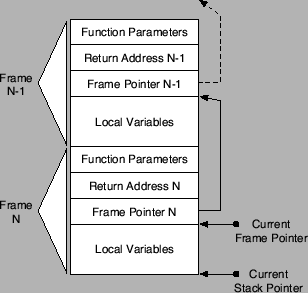
\includegraphics[width=0.7\linewidth]{stackframe.png}
%\end{center}

  ¿Donde se alojan los parámetros? ¿Y las variables locales? ¿Y la dirección de retorno?
  ¿Donde se aloja el enlace estático? ¿Que es el enlace estático?
  \item 
  ¿Que relación existe entre la forma en la que se guarden las variables y parámetros y la 
  presencia de recursividad en el lenguaje? ¿Como se relaciona esto mismo con la reentrancia?
  \item 
  En la llamada a un método en un lenguaje orientado a objetos 
  (por ejemplo C++), 
  ¿Donde se almacena la referencia al objeto actual asociado con el método?
\end{enumerate}


\item
La siguiente gramática no es LR(1).
\begin{verbatim}
[~/srcPLgrado/jison/jison-nolr]$ cat confusingsolvedppcr.y
%%
A: 
    B 'c' 'd' 
  | E 'c' 'f' 
;
B: 
    'x' 'y'
;
E: 
    'x' 'y' 
;

%%
\end{verbatim}
Encuentre una gramática Jison sin conflictos equivalente a la anterior.


\item
La siguiente gramática Jison presenta conflictos reduce-reduce:

\begin{verbatim}
[~/srcPLgrado/jison/jison-reducereduceconflict]$ cat reducereduceconflictPPCR2.y
%token ID

%%

def:    param_spec return_spec ','
        ;
param_spec:
             type
        |    name_list ':' type
        ;
return_spec:
             type
        |    name ':' type
        ;
type:        
             ID
        ;
name:        
             ID 
        ;
name_list:
             name
        |    name ',' name_list
        ;
%%
\end{verbatim}
Este es el diagnóstico de Jison:
\begin{verbatim}
~/srcPLgrado/jison/jison-reducereduceconflict]$ jison reducereduceconflictPPCR2.y
Conflict in grammar: multiple actions possible when lookahead token is ID in state 5
- reduce by rule: name -> ID
- reduce by rule: type -> ID
Conflict in grammar: multiple actions possible when lookahead token is : in state 5
- reduce by rule: name -> ID
- reduce by rule: type -> ID
Conflict in grammar: multiple actions possible when lookahead token is , in state 5
- reduce by rule: name -> ID
- reduce by rule: type -> ID

States with conflicts:
State 5
  type -> ID . #lookaheads= ID : ,
  name -> ID . #lookaheads= ID : ,
\end{verbatim}
Encuentre una gramática equivalente a la anterior sin conflictos.


\item
El lenguaje $\{ a^n b^n c^n / n \in \mathcal{N} \}$ no puede ser 
expresado mediante una gramática independiente del contexto.
Escriba un PEGJS (sin acciones semánticas)
que reconozca dicho lenguaje.
 

\end{enumerate}

